\documentclass{article}
\usepackage[utf8]{inputenc}
\usepackage{amsmath}
\usepackage[]{algorithm2e}
\usepackage{graphicx}
\usepackage{subfig}
%\usepackage{algorithm}
%\usepackage{algpseudocode}



\title{Framework and Simple tracking 3D}

\begin{document}

\maketitle	

The current version of the framework is shown in the Figure~\ref{fig:diagram}.

\begin{figure}[!h]
	\centering
    \centerline{\includegraphics[width=40em]{images/diagram.png}}
    \caption{Framework.}
    \label{fig:diagram}
\end{figure}

All framework is organized in 3 main objects, Strategy, Action and ObjectAction. The Strategy works like the "Command" pattern of GoF`s design patterns. In the implementation example of the tracking using this structure, the way that Strategy call the actions and how actions work together is similar to the pattern "Chain of Responsibility" of GoF`s design patterns. The exchange of data between the actions is made using a Context, who implements each interface required for each action.

The first version of the example using the framework is shown in the Figures~\ref{fig:f1},~\ref{fig:f2},~\ref{fig:f3} and~\ref{fig:fn}. A simple viewer was developed to get this visualization. One sphere is drawn in the position of each cell tracked, with a diameter of the max width of the cell. Each sphere is drawn using a different color. The viewer draws the cell in the last position with white color and a line linking the last position to the current one. Transformations in the camera is also provided.

In this first example, the cells in the frame t are being linked to someone in the frame t+1. A cost matrix is built and solved, after that the link is done. Missing cells are saved and when a splitting or division happen they are linked to one cell left. Left cells are linked to closest missed one, if there is someone, or to the closest one in the last frame. No other event is being processed for now. Some strange links are observed in the Figures~\ref{fig:f1},~\ref{fig:f2},~\ref{fig:f3} and~\ref{fig:fn}. This is happening because even the distance is too big one link is done between cells. For example, one cell could be alone because of some overlap, however if other cell goes in to the scene a link can be done between these 2 outliers.

For now, I am trying print the tracking in the same format required in the challenge, using the Amal`s implementation. I am also improving the algorithms.

\begin{figure}[!hbt]
	\centering
    \centerline{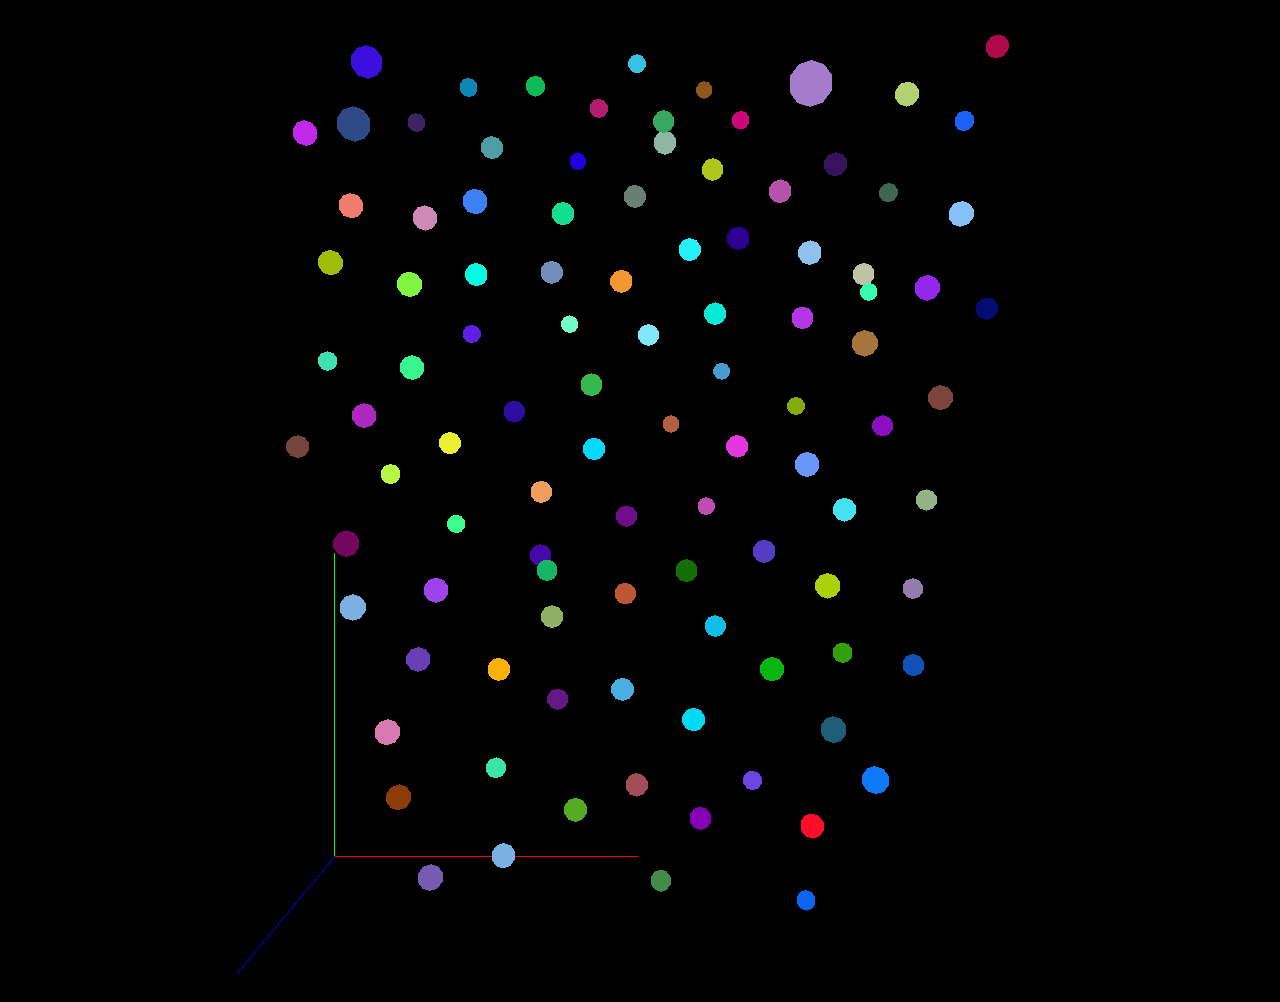
\includegraphics[width=40em]{images/f1.png}}
    \caption{Frame 1.}
    \label{fig:f1}
\end{figure}

\begin{figure}[!hbt]
	\centering
    \centerline{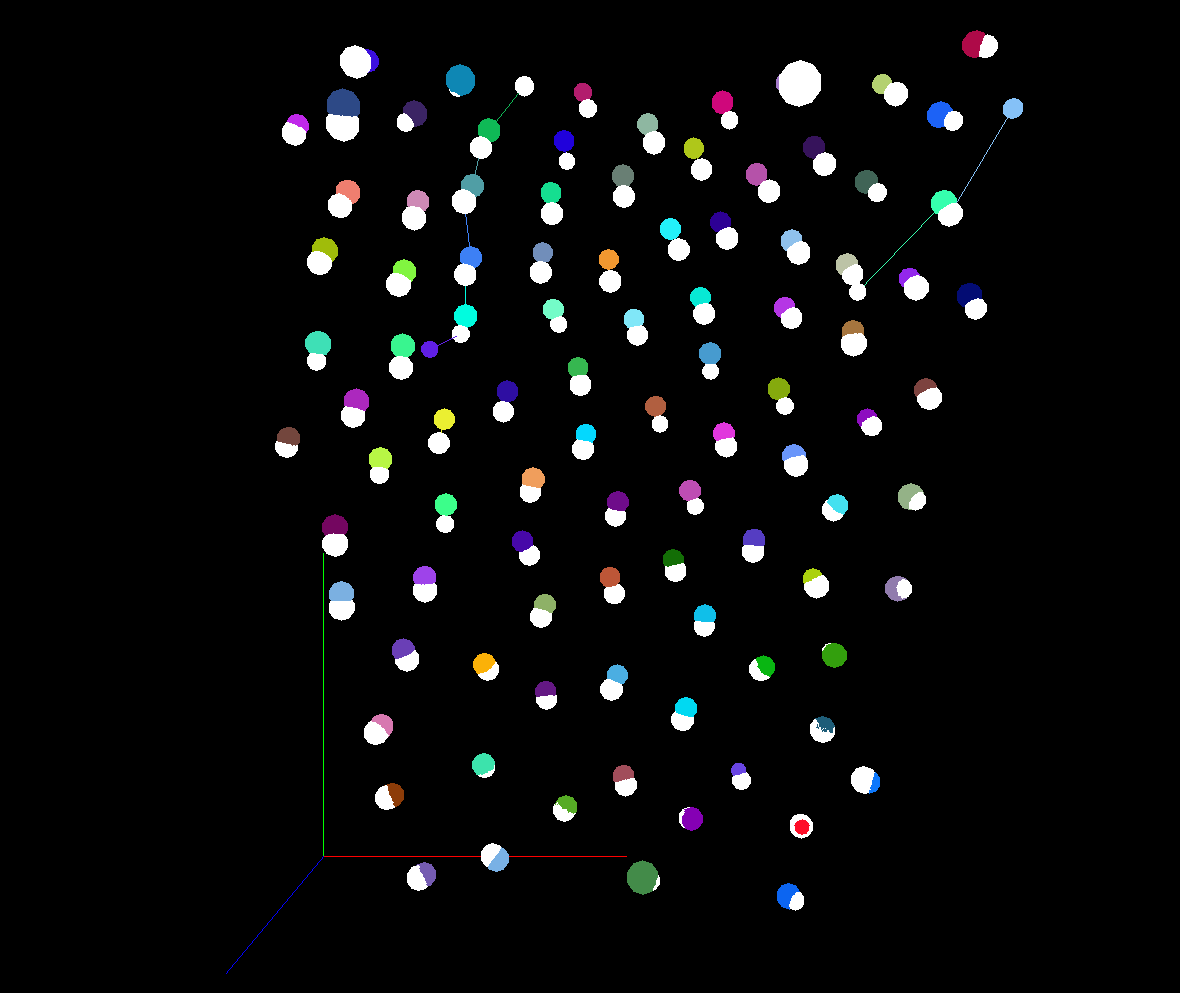
\includegraphics[width=40em]{images/f2.png}}
    \caption{Frame 2.}
    \label{fig:f2}
\end{figure}

\begin{figure}[!hbt]
	\centering
    \centerline{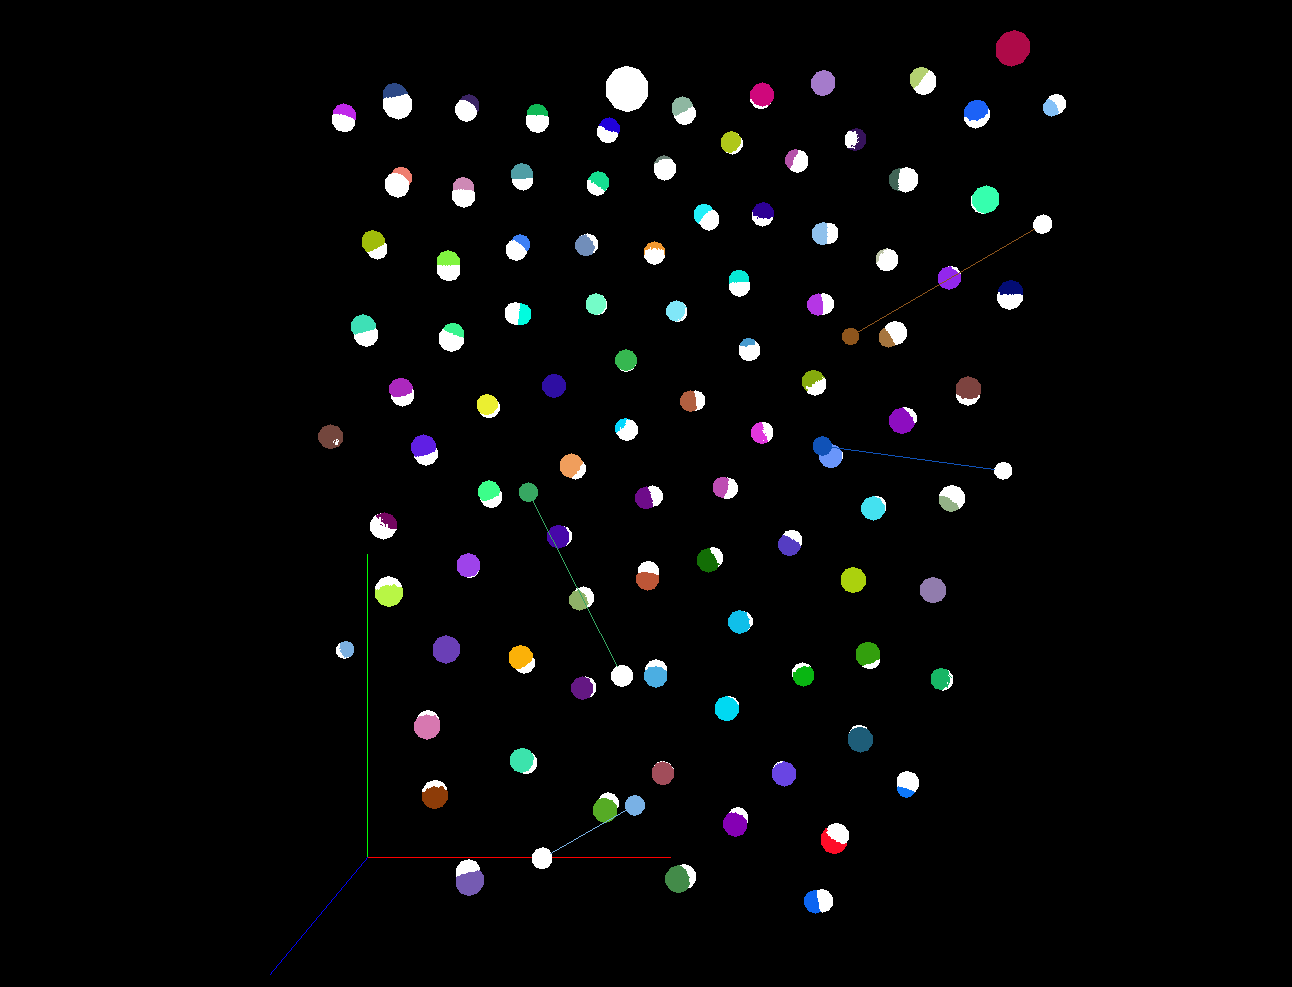
\includegraphics[width=40em]{images/f3.png}}
    \caption{Frame 3.}
    \label{fig:f3}
\end{figure}

\begin{figure}[!hbt]
	\centering
    \centerline{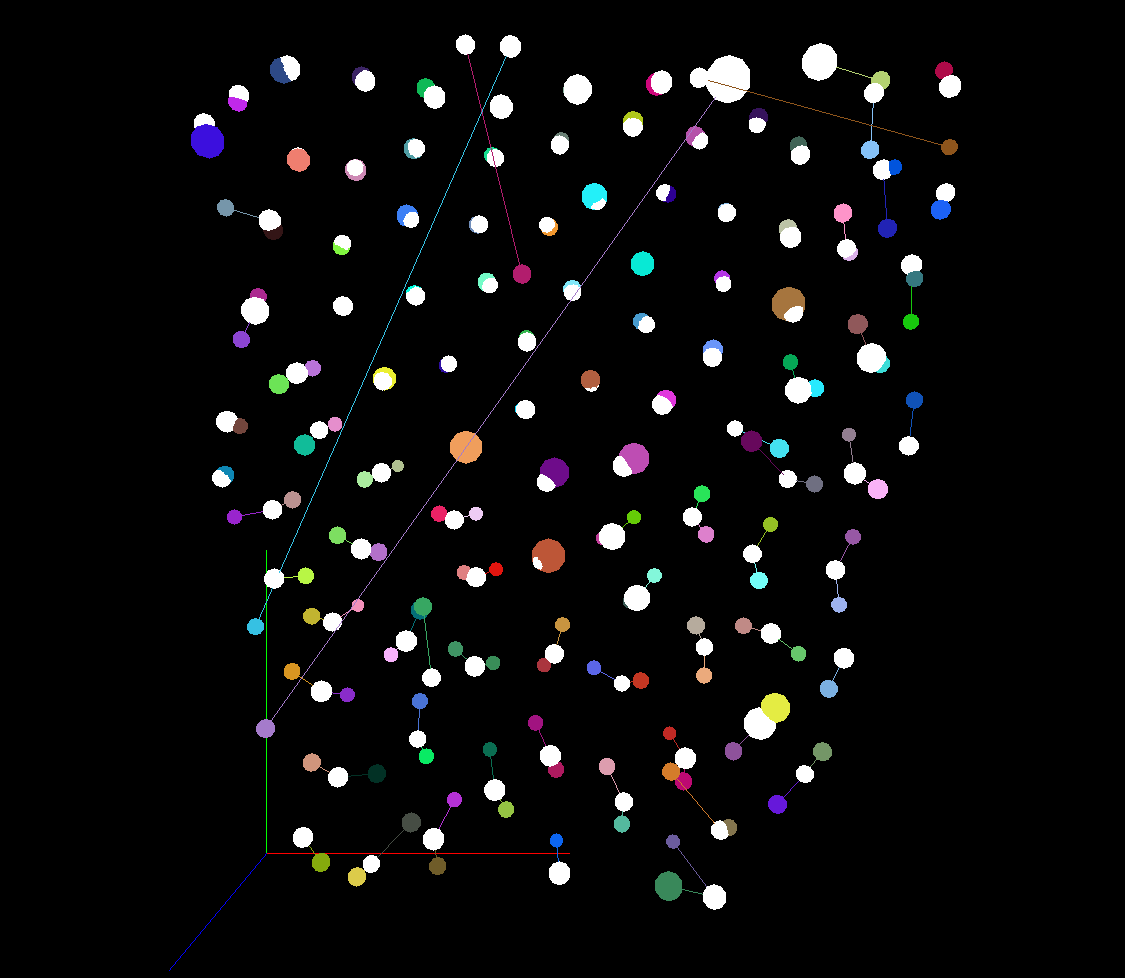
\includegraphics[width=40em]{images/f4.png}}
    \caption{Frame N.}
    \label{fig:fn}
\end{figure}

%
%\begin{algorithm}[H]
% \KwData{A set \(I\) of 2D images, where each image represents the features of the cells on the time \(t\).}
% \KwResult{A set \(L\) of lists, where each element \(t\) of each list \(L_i\) have the position of the cell \(i\) on the time \(t\)}
% $I\gets loadVideo()$ \;
% $T\gets \text{number of elements in } I$ \;
% $t\gets 1$ \;
% $P_t \gets \text{set of particles in the image } I_t$ \;
% \For{\text{each list i in } \(L\)} 
% {
%   $\text{ add the element i of } P_t \text{ to } L_i$
% }
% \For{t=2 to t=T} 
% {
% $P_t \gets \text{set of particles in the image } I_t$ \;
%	 \For{\text{each element i in } \(L\)} 
%	 {
%		  $c \gets \text{ the element of } P_{t} \text{ where the distance is the smallest to element t-1 in } L_{i}$
%		  $\text{ add c in } L_i$
%	 }
%	 \If{any element left in \(P_{t}\) }{
%		 $R \gets \text{list of elements left in } P_{t}$ \;
%		  \For{\text{each element k of } \(R\)} 
%		   {
%		  	 $c \gets \text{ the element t-1 of any list } L_{i} \text{ where the distance is the smallest to element k in } R $
%		  	 $e \gets \text{ the element t of the list } L_i $ \;
%		  	 $\text{ remove the element t from } L_i $ \;
%		  	 $\text{ create 2 new list } L_{i+1} \text{ and } L_{i+2} \text{ in } L$ \;
%		  	 $\text{ add the element e to }  L_{i+1} $ \;
%		  	 $\text{ add the element k of R to } L_{i+2} $ 
%		   }
%	   }
% }
% \caption{Simple tracking cells}
%\end{algorithm}


 





%--------------------------------------------------------------------------------
%\section{First example}

%The well known Pythagorean theorem \(x^2 + y^2 = z^2\) was 
%proved to be invalid for other exponents. 
%Meaning the next equation has no integer solutions:

%\[ x^n + y^n = z^n \]


%--------------------------------------------------------------------------------

%\section{Second example}

%In physics, the mass-energy equivalence is stated by the equation $E=mc^2$, discovered in 1905 by Albert Einstein.

%The mass-energy equivalence is described by the famous equation
%$$E=mc^2$$
%discovered in 1905 by Albert Einstein. 
%In natural units ($c$ = 1), the formula expresses the identity
%\begin{equation}
%E=m
%\end{equation}

%\section{Third example}

%This is a simple math expression \(\sqrt{x^2+1}\) inside text. 
%And this is also the same: 
%\begin{math}
%\sqrt{x^2+1}
%\end{math}
%but by using another command.

%This is a simple math expression without numbering
%\[\sqrt{x^2+1}\] 
%separated from text.

%This is also the same:
%\begin{displaymath}
%\sqrt{x^2+1}
%\end{displaymath}

%\ldots and this:
%\begin{equation*}
%\sqrt{x^2+1}
%\end{equation*}



\end{document}
